\chapter{PROCEDIMENTOS METODOLÓGICOS}

Nesse item serão apresentados aspectos metodológicos referentes a
presente pesquisa.

\section{TIPO DE PESQUISA}

O método de pesquisa utilizado no presente trabalho é de caráter pratico. Ele é descrita por Marconi e Lakatos (2017) como a busca por solução de problemas que ocorrem na realidade a partir da aplicação prática de resultados, que obviamente são gerados através de um conhecimento prévio. Através do fluxograma que se segue na Figura 4.1, é possível entender o processo utilizado para a realização da pesquisa.\bigskip

\begin{figure}[!ht]
	\centering
	\caption{Fluxograma da pesquisa.}
	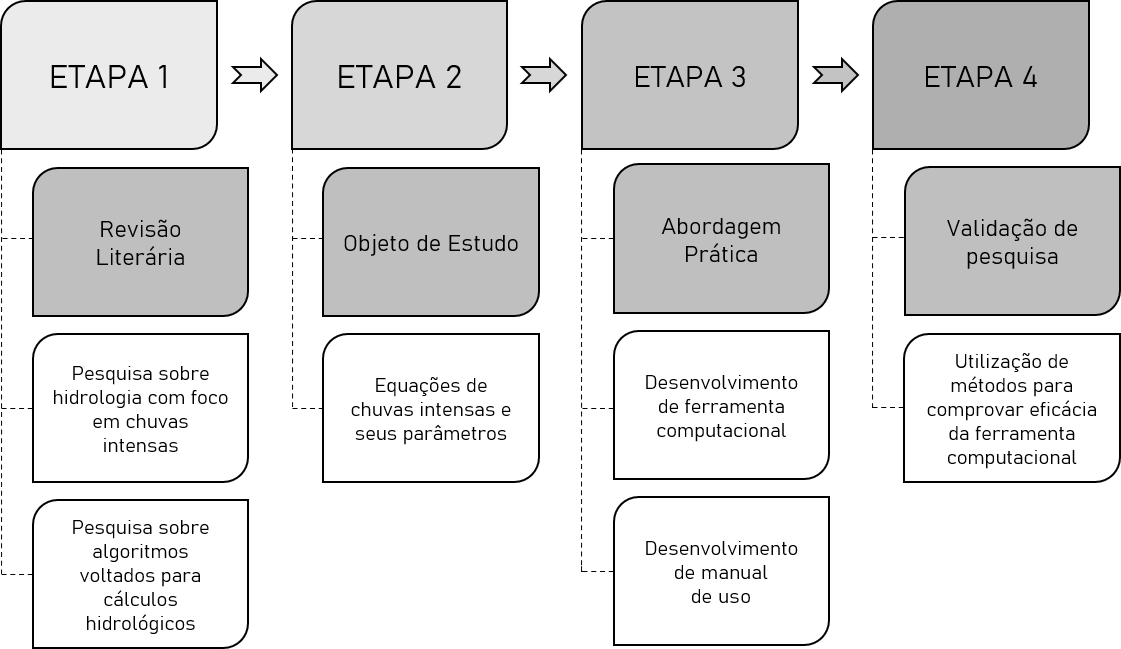
\includegraphics[width=.7625\linewidth]{figuras/fluxograma_de_pesquisa.png}
	\caption*{\textbf{Fonte:} De autoria própria (2023).}
	\label{fig:fluxograma_de_pesquisa.png}
\end{figure}

%\section{OBJETO EM ESTUDO}

\section{MÉTODOS}

Para alcançar boas soluções na determinação da equação de chuvas intensas e seus parâmetros, de acordo os dados de precipitação utilizados, foi desenvolvida uma ferramenta computacional que cumpre essa finalidade.

\subsection{A interface}

O desenvolvimento se iniciou na elaboração de uma interface gráfica que permite a interação do usuário com à máquina, de forma que ele preencha a ferramenta computacional com todos os dados que se necessitam para a elaboração da equação, através do calculo de seus parâmetros. É importante ter em mente, que durante o desenvolvimento da interface, priorizou-se a simplificação das funções de interação da ferramenta, visando torna-la intuitiva e de fácil compreensão, possibilitando um rápido aprendizado de uso.

A interface gráfica foi criada através da linguagem de programação Python, explicada no referencial teórico. Para o seu desenvolvimento, foi utilizado o Tkinter, que é uma biblioteca nativa do próprio Python. Ele permite a criação de telas, botões, tabelas, além de outras ferramentas. Através delas é possível a interação do usuário, pois todas as suas solicitações passam primeiramente por elas.

\subsection{Os algoritmos de armazenamento e tratamento de dados}

O calculo da ferramenta computacional foi desenvolvido em duas direções, uma delas através de dados fornecidos pelo calculista, nomeada de independente para um melhor entendimento. A outra a direção segue a partir de um banco de dados prévio, sendo chamada de dependente. Fica claro então que para que ocorram os cálculos, são necessários dados.

Sabendo disso, de início foi programado um banco de dados com informações de precipitações diárias de postos pluviométricos que se estendem por todo o território da Paraíba. Sua escolha se deu devido a precisão e vastidão das informações, disponibilizadas pela Agência Executiva de Gestão das Águas do Estado da Paraíba (AESA), com séries históricas que variam entre os anos de 1994 e 2022.

Para esses dados, foram desenvolvidos um mapa interativo da Paraíba na interface gráfica, que tem seu território traçado a partir de sua latitude e longitude, e um algoritmo de interpolação de dados. Nesse mapa, ao selecionar uma determinada coordenada, é feito uma interpolação das precipitações diárias pelo método IDW, a partir dos cinco postos pluviométricos mais próximos que possuem a mesma quantidade de anos iguais. Assim, a coordenada selecionada passa a ter uma série histórica interpolada de precipitações diárias. 

Também foi elaborado uma lista dos postos pluviométricos fornecidos pela AESA. Tudo isso para que seja possível calcular as equações IDF desses locais. Entende-se então, que é possível replicar isso para outras regiões do globo, desde que se tenha os dados delas. 

Outra parte importante da ferramenta, está no algoritmo que permite a conversão de séries de precipitações diárias de vários anos, em séries de precipitações máximas diárias anuais. Ele auxiliará no tratamento dos dados interpolados do mapa paraibano, dos postos pluviométricos da Paraíba, e dos dados informados pelo usuário, de séries de precipitação de chuvas diárias de vários anos, para preenchimento de falhas.

No que tange preencher os dados faltantes, foi programado um limiar de falhas, onde caso um determinado ano tenha dias sem informações que ultrapassem esse limite, ele será desconsiderado. Estando dentro do limiar, o usuário escolherá se haverá a exclusão dos dados falhos, ou interpolação pelo método IDW das precipitações máximas diárias mensais dos dados informados, para que assim se obtenha as precipitações máximas diárias anuais.

\subsection{Os algoritmos de cálculo}

Tratando dos cálculos, o algoritmo que verifica se há tendência nas séries de precipitações máximas diárias anuais foi programado a partir das bibliotecas NumPy e pyMannKendall, estando a segunda delas disponível no PyPi, que é um repositório oficial de bibliotecas de terceiros do Python. 

Os algoritmos de distribuições de probabilidade, testes de aderência e métodos de otimização tiveram como bibliotecas em seus desenvolvimentos o SciPy e o NumPy, com exceção da distribuição de Gumbel e do método dos mínimos quadrados que se utilizaram apenas da segunda citada. Os algoritmos de análise de precisão dos parâmetros da equação IDF foram desenvolvidos utilizando a biblioteca NumPy. Já o algoritmo de desagregação das chuvas não necessitou de nenhuma biblioteca específica além do ambiente padrão de desenvolvimento do Python.

A integração desses algoritmos possibilita a escolha por parte do usuário, dos tempos de retorno, durações, distribuição de frequência, teste de aderência e método de otimização, para o cálculo dos parâmetros da equação das chuvas intensas. Também é possível ajustar os intervalos ou números de partida dos métodos de otimização, para torna-los ainda mais precisos, além das funções que possibilitam a escolha dos melhores ajustes, onde a ferramenta calcula todas as combinações possíveis para determinar a equação IDF mais precisa.

Deu-se então a implementação de todos esses códigos na interface gráfica, permitindo ao usuário chegar aos parâmetros da equação IDF de três formas, duas delas se direcionando de maneira dependente, e uma independente. Quando o usuário decide pela interpolação das coordenadas do mapa da Paraíba, ou pela escolha de algum posto pluviométrico da lista que permeia o território paraibano, o direcionamento é dependente. Já quando o usuário fornece sua própria série histórica de precipitações diárias, a direção é independente. 

\subsection{Os arquivos de instalação e guias de uso da ferramenta computacional}

Foi escrito um manual de uso prático da ferramenta. Contudo, dentro da desta, também foram criados guias básicos de ajuda, além de como acessar seu repositório de códigos e o referencial teórico que guiou sua criação. Após finalizar toda sua programação, foi desenvolvido um arquivo executável com a biblioteca PyInstaller e um instalador com o programa Inno Setup, com a finalidade de facilitar o acesso à ferramenta para as pessoas que possuem menos familiaridade com linguagens de programação, em específico o Python.

\subsection{O código fonte da ferramenta computacional}

Para que haja a possibilidade de estudos posteriores, adaptações, correções, e até mesmo melhoramentos e evoluções, todo o código fonte da ferramenta computacional foi disponibilizado no GitHub. A intenção é fomentar o desenvolvimento científico, e facilitar a compreensão de tudo que foi elaborado.

%\section{ASPECTOS ÉTICOS}

%\section{TRATAMENTO DOS DADOS}